\section{SMB protocol}
Before entering in the details of the exploit, it is important to describe what is the SMB 
protocol and how it works.
The Server Message Block (SMB) is a procol based on TCP/IP used for file sharing and printer sharing 
in a computer network.

\subsection{Microsoft Windows implementation}
The SMB is used in Microsoft Windows systems since 1996 in two services for using the computer as a 
workstation or a server.
During the time a lot of versions of SMB suceedes, in this section it will be analyzed only the first version, because
this is the one involved in the vulnerability.\\
The Windows implementation of SMB version 1 is an extension of the already existing Common Internet File System (CIFS)
which was the network file-sharing protocol for Windows NT.
SMB added some features on security and disk management, but most importantly it substituted the old NetBios service with an entire 
TCP connection.\\
In the SMB V1 there are three phases\cite{microsoft-smb}:
\begin{itemize}
    \item Establishing a TCP session
    \item Negotiating a Dialect
    \item Establishing an SMB connection
    \item Accessing Resources
\end{itemize}
It is important to notice that during the establishing of the SMB connection the client and server decide which is the maximum
buffer size for each SMB message (also called transaction).
The Windows Server that receives the SMB request has a driver caled Srv.sys that aims to load balance the queue of the SMB commands received.

\subsection{Structure}
The SMB packets are divided into three parts: Header, Parameter Block and the Data block.\\
The Header block has the following parts\cite{microsoft-smb}:
\begin{itemize}
    \item Command: SMB query to run into the server
    \item Flags: it indicates if it is a response or a request
    \item Errno: error number
    \item Signature
    \item Identifiers (PID, ID, RID, UID)
\end{itemize}
The Parameter block is used to specify the parameters values of the commands in the header. The last block instead regards 
all the data of the packet.
\begin{figure}[ht!]
    \centering
      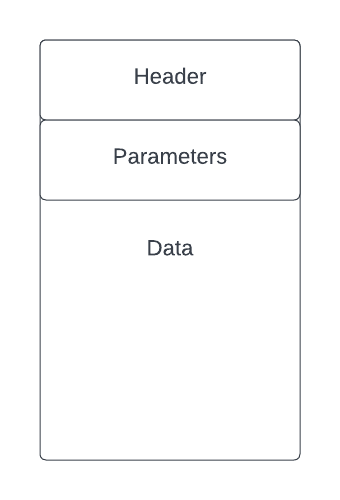
\includegraphics[]{images/smb_structure.png}
      \caption{SMB packet structure}
\end{figure}

\subsection{Transactions}

The accessing of resources is done with Transcations, which are SMB messages that enables atomic read and write
between client and server.
From a packet view, they are just an SMB messages that embeds another SMB message in the data block.
\begin{figure}[ht!]
    \centering
      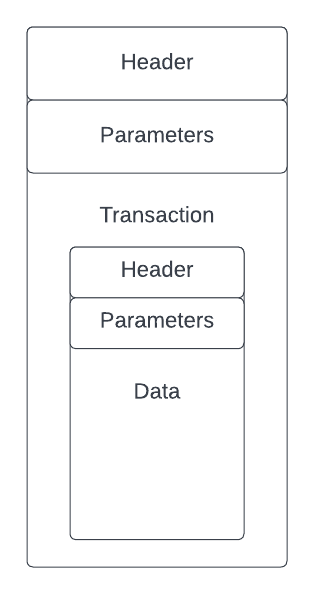
\includegraphics[scale=0.5]{images/smb_trans_structure.png}
      \caption{SMB transaction packet structure}
\end{figure}

In each Transaction there are the following parameters\cite{microsoft-transactions}:
\begin{itemize}
    \item Offset: indicates when the data block begins
    \item Count
    \item TotalCount
    \item Displacement: It indicates where start writing in the srv buffer
\end{itemize}

When a Transaction has a data block bigger then the maxBufSize specified in the connection establishment, the server requests some Transaction Secondary in order
to complete the data transfer\cite{microsoft-transactions}.
There are different kind of this Transaction Secondary due to the different versions of the SMB implementation like Transaction2, TransactionSecondary or NTTransaction2.
\begin{figure}[ht!]
    \centering
      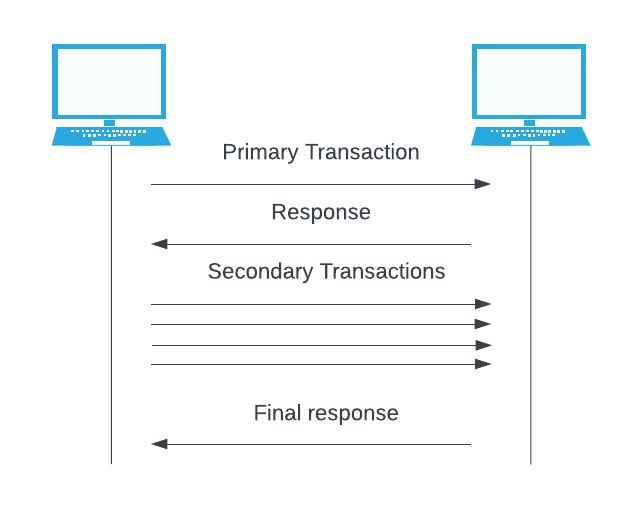
\includegraphics[]{images/transactions_scheme.png}
      \caption{Transactions exchange scheme}
\end{figure}